
\chapter{مقدمه}

\section{؟}

امروزه روش‌های بازاریابی برای انواع محصولات و خدمات مختلف،‌ با زمان‌های قدیم متفاوت شده است. در بسیاری از روش‌های بازاریابی سنتی و قدیمی، محصول و خدمت ارائه شده در جایگاه اصلی قرار می‌گیرد و چندان به نیاز مشتری توجهی نمی‌شود. از طرفی اگر نیازمندی‌های مشتری مطرح شوند، به آن‌ها به چشم یک بهبود برای نسخه‌های بعدی محصول یا خدمت ارائه شده نگاه می‌شود و اساسا ارائه دهنده آن محصول یا خدمت، ممکن است تفاوت‌های شخصی مشتریان خودش را تا حد موردنیاز درک نکند\cite{marketing2}.

اما در روش‌های نوین، از همان ابتدای بازاریابی، جامعه هدف بطور صریح‌تر و محدودتری مشخص می‌شود و اگر فردی درون و یا نزدیک به مرزهای این جامعه قرار نگیرد، برای صرف هزینه بازاریابی اولویت نخواهد داشت و هزینه و وقتی که در روش‌های قدیمی صرف جذب او برای استفاده از خدمت یا محصول ارائه شده می‌گشت، صرف افراد درون جامعه هدف می‌شود تا بازدهی بهتری داشته باشد.

یکی از روش‌هایی که روز به روز درحال رشد و استفاده بیشتر در بین ارائه‌دهندگان خدمات و محصولات است که شناسایی این جامعه هدف را بطور هرچه دقیق‌تر و سریعتر میّسر می‌کند، روش‌های نوین سنجش علاقه‌مندی افراد نسبت به موضوعات مختلف است که با اعمال برخی تکنیک‌های داده‌کاوی و یادگیری ماشین،  می‌توان بطور دقیق‌تری نسبت به آنچه در روش‌های سنتی در جریان است، نسبت به علاقه‌مندی افراد به محصولات یا خدمات دیگر پیش‌بینی داشت\cite{marketing3}.

همانطور که در شکل
\cref{fig.1}
نمایش داده شده است، در روش مبتنی بر حساب کاربری بدلیل تولید سوابق علاقه‌مندی توسط مشتری، امکان شخصی‌سازی بسیار بهتر خدمات از همان ابتدا فراهم می‌شود؛ برخلاف روش بازاریابی سنتی که در آن به مرحله شناسایی جامعه دقیق هدف در آخرین اولویت قرار دارد.\\

\begin{figure}[H]
	\centering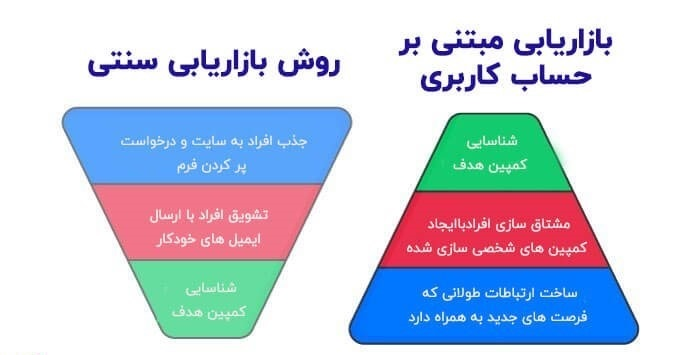
\includegraphics[scale=0.7]{marketing}
	\caption{مقایسه شیوه بازاریابی سنتی و مدرن\cite{marketingimage}}\label{fig.1}
\end{figure}
\newpage

درواقع سنجش علاقه‌مندی مشتریان به محصولات و خدمات مشابه و همگروه با محصولات ما، یکی از مهم‌ترین ابزارهایی است که ورودی‌های موردنیاز را برای پیش‌بینی آتی از علاقه‌مندی‌های آن مشتریان فراهم می‌کند و در نتیجه، با استفاده از الگوریتم‌های مختلف موجود در این حوزه، می‌توان به ارائه پیشنهادات مرتبط به آنان پرداخت.\\

بطورکلی، یکی از روش‌های بهبود این نوع بازاریابی، استفاده از مکانیزم‌های خودکنترلی‌ست. به این معنا که خروجی‌های این روش (که شامل پیشنهادات به مشتریان است)، با علاقه‌مندی‌های بعدی آن‌ها مقایسه می‌شود و از این طریق، میزان دقت سامانه در پیش‌بینی داده شده مشخص شده و تغییرات خودکاری در جهت بهبود سامانه تولید پیشنهادات در آن ایجاد می‌شود. این روش خودکنترلی بسیار شبیه به آن چیزی است که امروزه در فرآیند آموزش شبکه‌های عصبی رخ می‌دهد که درحال حاضر جزئیات آن از حوصله این موضوع خارج است و به ذکر همین مقدار از ارتباط آن به این موضوع بسنده می‌کنیم\cite{marketing1}.\\

%\section{خدمات مبتنی بر مکان}
%\subsection{خدمات حضوری}

روزانه حجم بسیار زیادی جابجایی جمعیت درون شهری، چه بصورت پیاده و چه بصورت سواره صورت می‌گیرد. آن‌چه که بطور معمول برای افراد درون این جمعیت مهم است، مقصد جابجایی آن‌هاست، و نه مسیر جابجایی.\\

بسیاری از خدمات امروزه بر بستر اینترنت و بصورت مجازی ارائه می‌شوند؛ اما همچنان تعداد ارائه‌دهندگان خدمات حضوری بسیار قابل توجه است؛ از رستوران‌ها تا انواع فروشگاه‌ها. با استناد به آمار خریدهای حضوری و آنلاین و مقایسه آن‌ها در
\cref{fig.2}
و با عنایت به این‌که تفاوت این دو آمار در کشور ایران بیشتر از کشور ایالات متحده آمریکاست در می‌یابیم همچنان مردم بجز درمورد برخی دسته از محصولات، اکثر خریدهای حضوری را به مجازی ترجیح می‌دهند\cite{marketing4}.\\

\begin{figure}[H]
	\centering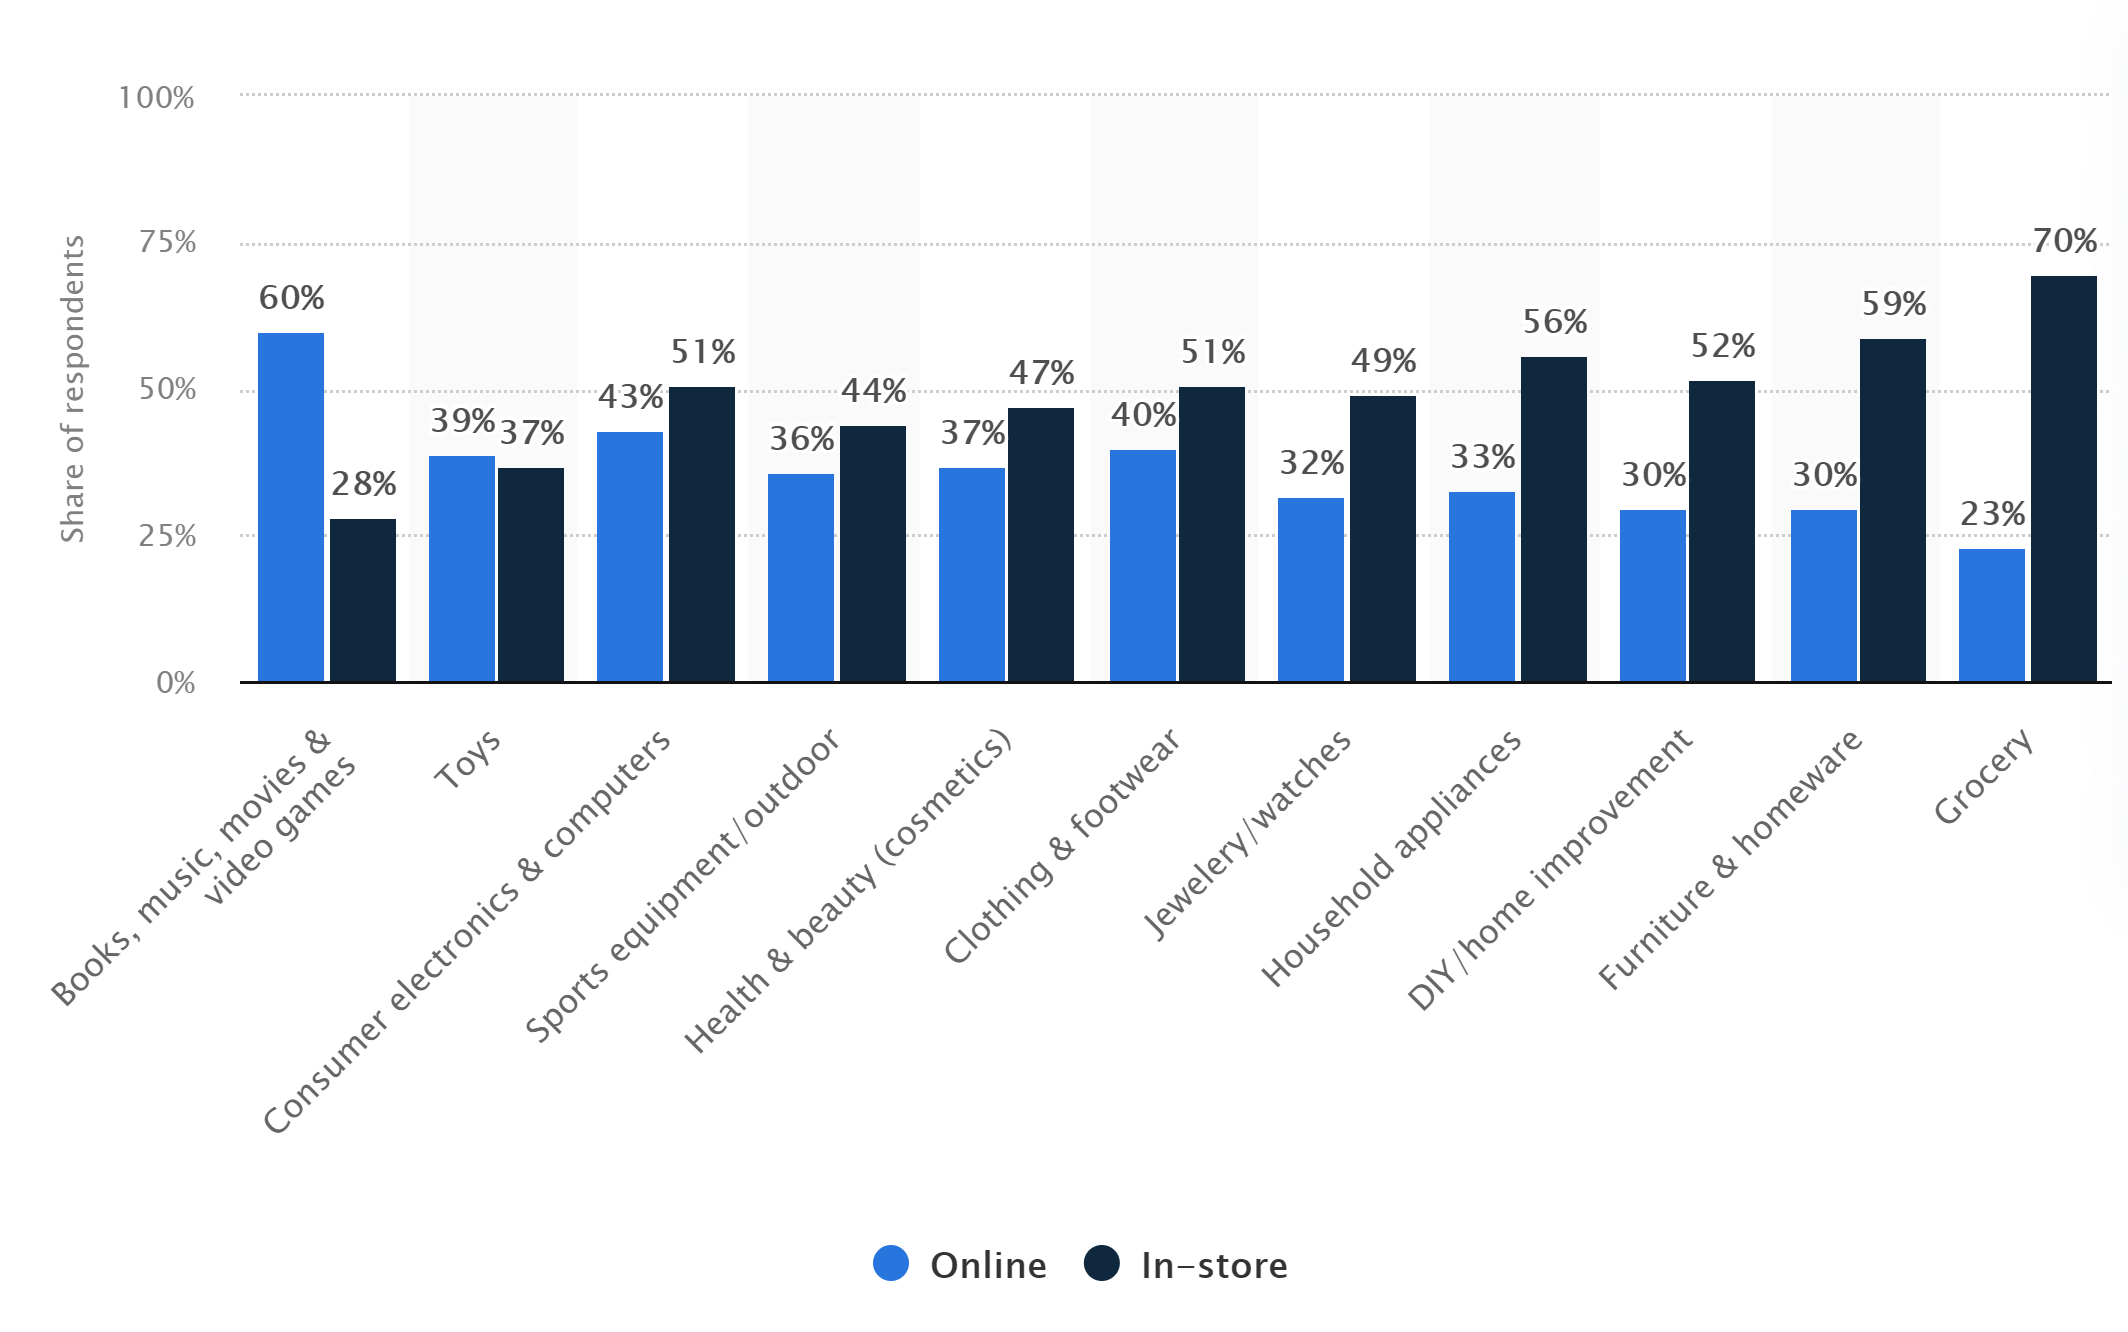
\includegraphics[scale=.4]{ecomm-prefer}
	\caption{مقایسه آمار خریدهای حضوری و مجازی در ایالات متحده آمریکا، ۲۰۱۷\cite{marketing4}}\label{fig.2}
\end{figure}

از مهم‌ترین دلایل مردم برای انتخاب خرید حضوری در مقابل خرید مجازی می‌توان به عدم توانایی تست محصولات و بررسی فیزیکی آن‌ها، عدم وجود تجربه خرید حضوری در خریدهای مجازی و ترس از خرابی محصولاتی که بصورت مجازی خریداری می‌شوند عنوان کرد که در
\cref{fig.3}
به دلایل دیگر و سهم هرکدام اشاره شده است.\cite{marketing5}
\begin{figure}[H]
	\centering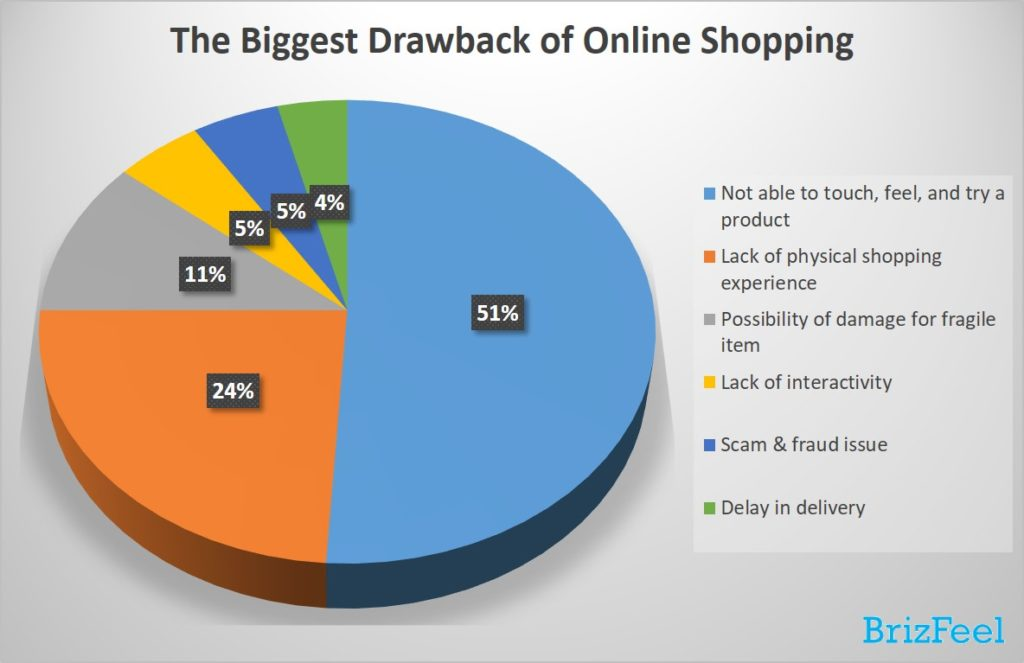
\includegraphics[scale=.5]{online_drawbacks}
	\caption{مهمترین دلایل ترجیح خرید حضوری به مجازی\cite{marketingimage2}}\label{fig.3}
\end{figure}
\newpage

%\subsection{خدمات و جابجایی مکانی}

کمتر مسافر درون‌شهری را می‌توان یافت که به مسیر جابجایی خود در طول شهر، به اندازه مقصد و یا حتی بیشتر از آن اهمیت بدهد! یکی از دلایل این امر، عدم اطلاع به موقع افراد از اماکن و فروشگاه‌ها و بطورکلی انواع خدمات موجود در آن مسیر است. حتی اگر آن‌ها را از قبل بشناسند، عموم مردم بدلیل مشغله روزمره، وجود آن‌ها را در هنگام عبور از نزدیکی‌شان فراموش می‌کنند.\\

اگر سامانه‌ای وجود داشته باشد که بتواند با تکیه بر داده‌های مرتبط با موقعیت مکانی کاربر، پیشنهاداتی را مبتنی بر دیگر خصوصیات شخصی به او ارائه کند، می‌تواند بازار خوبی در بین جمعیت داشته باشد. در این سامانه، فروشندگان با ارائه محصولات خود، زمینه اعلام علاقه‌مندی کاربران را به آن‌ها فراهم می‌کنند؛ از طرف دیگر،‌ کاربران می‌توانند مطابق با موقعیت مکانی خود، از نزدیک‌ترین پیشنهاداتی که این پلتفرم به آن‌ها می‌دهد مطلع شده و درصورت تمایل برای بازدید و خرید اقدام کنند.

%\section{روند کلی پروژه}
%\subsection{هدف پروژه}

هدف از این پروژه، طراحی سامانه‌ای است که بتواند با توجه به ویژگی‌های هر کاربر، تخفیفاتی برای خرید محصولات فروشگاه‌های عضو سامانه را به او پیشنهاد کند؛ اصلی‌ترین ویژگی مورد توجه، موقعیت مکانی  کاربر است که سامانه‌ با استفاده از آن می‌تواند پیشنهادات مبتنی بر مکان  به کاربر ارائه دهند. ویژگی دیگر مورد استفاده، اعلام علاقه‌مندی یک کاربر به خدمات مشابه یک خدمت پیشنهادی است که در سامانه مورد استفاده قرار خواهد گرفت.\\

از طرف دیگر، ارائه کنندگان محصولات (فروشندگان کالا) اقدام به ثبت موقعیت مکانی، زمینه محصولات خود و جزئیات آن‌ها، بهمراه کدهای تخفیفی برای خرید آن محصولات در سامانه کرده تا به کاربرانی که ممکن است از نزدیکی آن فروشگاه عبور کنند و احتمالا به آن محصولات علاقه دارند، اطلاع داده شود.\\

\newpage

%\subsection{اجزاء پروژه}

پیاده‌سازی این پروژه بطورکلی شامل 3 بخش می‌شود:
\begin{enumerate}
	
	\item سامانه اصلی، که وظیفه نگهداری داده‌ها (از جمله خصوصیات کاربران و فروشندگان) و همچنین پردازش و تحلیل آن‌ها را برعهده دارد. بخش اصلی پروژه و تمرکز پیاده‌سازی همین قسمت است؛ اما بدلیل اینکه برای عملکرد صحیح و کامل این سامانه، باید رابط‌های کاربری ویژه کاربران ایجاد شود، دو بخش دیگر نیز وجود خواهد داشت.
	
	\item نرم‌افزار گوشی هوشمند  برای کاربران (فروشندگان و خریداران): این نرم‌افزار که برای گوشی‌های هوشمند بر بستر اندروید  طراحی می‌شود، برای دریافت خدمات سامانه توسط هر دو گروه کاربران می‌باشد. در این نرم‌افزار باید قابلیت‌های یک نرم‌افزار اطلاع‌رسانی تخفیف‌های فروشگاهی موجود باشد، و علاوه بر آن بتواند پیشنهادات را بر اساس تاریخچه موقعیت کاربر و علاقه‌مندی‌های قبلی او از سامانه اصلی دریافت کرده و به او نمایش دهد. همچنین برای فروشندگان باید قابلیت وارد کردن اطلاعات فروشگاه‌ها و جزئیات تحفیف‌های آن‌ها فراهم شود.
	
	\item پنل مانیتورینگ تحت وب (برای مدیران و ناظران سامانه): در این پنل، اطلاعات کاربران،‌ فروشگاه‌ها و محصولات آن‌ها بایستی قابل نمایش باشد تا ناظران سامانه بتوانند وضعیت فعلی کسب‌وکار خود را بهتر درک کرده و اقدامات کنترلی بهتری در سطح پلتفرم انجام دهند.

\end{enumerate}

لازم به ذکر است که در انجام این پروژه، تمرکز بر بخش نرم‌افزاری آن و چالش‌های معماری و الگوریتمی و فرآیندی بوده است و بخش مرتبط با تولید و ارائه پیشنهادات صرفا بصورت نمونه پیاده‌سازی شده و از الگوریتم‌های هوش مصنوعی و یادگیری ماشین در پیاده‌سازی آن استفاده نشده است. در واقع، رابط موردنیاز برای این الگوریتم‌ها طراحی شده که در آینده می‌توان با پیاده‌سازی انواع روش‌های مختلف و اتصال آن‌ها به رابط طراحی شده، از عملکرد آن در این سامانه استفاده کرد. در فصل انتهایی این سند پیشنهاداتی برای این بخش مطرح خواهد شد.
\newpage

%\subsection{پشته مورد استفاده برای پیاده‌سازی}

برای پیاده‌سازی اجزای مختلف این پروژه از ابزارها و پشته‌های مختلفی استفاده شده که در فصول بعدی بطور مفصل به دلایل انتخاب آن‌ها و نقش هرکدام اشاره خواهد شد؛ اما در اینجا و بعنوان مقدمه صرفا آن‌ها را نام می‌بریم:
\begin{itemize}
	\item \lr{Node.js (+ Typescript)}
	\item \lr{Apollo (+ Express)}
	\item \lr{GraphQL}
	\item \lr{MongoDB}
	\item \lr{Mocha (+ Chai)}				
	\item \lr{React Native}
	\item \lr{ReactJS}
\end{itemize}
